\documentclass[11pt]{article}
\usepackage[utf8]{inputenc}\usepackage[T1]{fontenc}\usepackage{lmodern}
\usepackage[margin=1in]{geometry}
\usepackage{microtype}\setlength{\emergencystretch}{3em}
\usepackage{amsmath,amssymb,amsthm,booktabs,graphicx,array,xcolor,enumitem,caption}
\graphicspath{{figures/}}
\usepackage[round]{natbib}
\usepackage[hidelinks]{hyperref}



  \newcommand{\priorp}{\citep{rathore2026coherent}}
  \newcommand{\priort}{\citet{rathore2026coherent}}


\title{\bf Scale Fixes Local Errors First: Differential Scaling\\of Chess Transformer Failures}


  \author{
    Mohit Pratap Singh Rathore\\ \small Oviqo Private Limited
    \and
    Gunveer Sinh Kalsi\\ \small Oviqo Private Limited
    \and
    Sriharsha Meduri\\ \small Oviqo Private Limited
  }

\date{}

\begin{document}
\maketitle

\begin{abstract}
Scaling reduces how often language models make long-horizon errors, but it is
rarely asked which errors it removes. We classify every illegal move made by
search-free chess transformers by what made it illegal, using only a rules engine,
and measure how the absolute rate of each class falls with model size. Across
18 models spanning 3.4M to 39.9M
parameters, errors decidable from the move's own squares fall with exponent
$-$0.574, while moves illegal only because they leave the king in
check fall with exponent $-$0.112: a paired differential of
+0.461 [+0.259, +0.599]. Failures
that occur despite correct internal belief about the move's squares do not fall
at all, exponent +0.023. The ordering replicates on an independent
character-level ladder spanning a 38-fold parameter range, and in
OthelloGPT every residual failure is of the non-local kind. A causal account
follows: belief is coupled to action locally, a repair edit can correct about two
squares, and the class that scale leaves behind is the class local correction
cannot reach. The standard intervention metric inverts on the same data. Illegal
move rate ranks a norm-matched random edit above correct repair in
18 of 18 models, because hedging lowers it. Finally, these
per-category fits and a separately fitted aggregate cannot both hold, since a sum of
power laws is not a power law; we derive the total from the categories instead.
\end{abstract}

\noindent\textbf{Keywords:} scaling, failure analysis, world models, state
tracking, chess, interpretability, evaluation methodology

% ====================================================================
\section{Introduction}

Scaling laws describe how aggregate loss falls with parameters and data
\citep{kaplan2020scaling,hoffmann2022training}. They say much less about the
composition of what remains. A model that makes half as many errors at ten times
the size may have removed every kind of error evenly, or removed one kind almost
entirely and left another untouched. The two cases recommend different research.
If scale removes errors evenly, more scale is the remedy for all of them. If it
removes some and not others, the ones it leaves are where effort should go, and
interventions aimed at the kind scale already removes are buying something that
arrives for free.

Long-horizon reasoning is where this question matters most and is hardest to ask,
because in open-ended text there is no ground truth for why a step was wrong. We
ask it where there is. A search-free transformer trained on chess move notation
produces a move at every position, a rules engine decides whether it is legal,
and when it is not, the same engine says why. Some illegal moves are decidable
from the two squares the move names: the source square is empty, or holds an
opponent's piece, or the destination holds one of the mover's own. Others turn on
the whole board: the move is geometrically possible for the piece but its path is
blocked, or it is pseudo-legal and rejected only because it leaves the king in
check. That distinction between local and global illegality is exact, needs no
model internals, and is the axis along which we measure scaling.

\paragraph{What we find.}
\begin{enumerate}[nosep]
\item \textbf{Failure classes scale at different rates, ordered by locality.}
Absolute rates of local errors fall steeply with size and global ones slowly. The
empty-source class falls 4.01-fold across our ladder and the
check class 1.31-fold, a differential exponent of
+0.461 that excludes zero in every rung resample. No probe,
intervention, or interpretability method enters this result.
\item \textbf{It is not an artefact of our models.} The same ordering holds on an
independent ladder with different data, notation, and training code, and in a
game whose legality is non-local by construction.
\item \textbf{The component scale does not remove is the one local correction
cannot reach.} Internal belief is causally coupled to action at the squares a
move touches, a residual-stream repair can install at most about two squares, and
failures that occur despite correct belief at those squares have an exponent
indistinguishable from zero.
\item \textbf{The usual way of scoring interventions reads this backwards.}
Illegal-move rate rewards edits that flatten the output distribution, and on our
data it prefers a random direction to the correct repair in every model.
\end{enumerate}

\paragraph{Contributions.}
A probe-free, rules-grounded measurement of how failure composition changes with
scale; its replication across two ladders and two games; a mechanistic account,
with a measured capability limit on the causal instrument; and a demonstration
that a widely used intervention metric is anti-correlated with the effect it is
meant to measure. The probe and edit instruments used in Section~\ref{sec:mech}
are established in prior work \priorp; here they serve only to
explain a result that stands without them.

% ====================================================================
\section{Related Work}

\paragraph{Scaling and what it leaves.}
Aggregate loss follows power laws in parameters, data, and compute
\citep{kaplan2020scaling,hoffmann2022training}. Decomposing an aggregate into
components with separate exponents is the step we take, applied to error classes
rather than to loss, in a domain where the classes are defined by an oracle
rather than by annotation.

\paragraph{World models in game transformers.}
Linear probes recover board state from move sequences \citep{li2023emergent},
with linear structure \citep{nanda2023emergent}; chess is an established
state-tracking testbed \citep{toshniwal2022chess}; and board-state probes in a
character-level chess model can be intervened on \citep{karvonen2024emergent},
later serving as ground truth for dictionary learning \citep{karvonen2024measuring}.
\citet{walker2026chess} benchmark exact state tracking across architectures at a
parameter range close to ours, \citet{li2026tracking} separate state tracking from
decision quality, and \citet{pereira2026transformers} and
\citet{harang2025tracking} document state decay over long generations. State
decay and chess state tracking are not our contribution; how the composition of
failure changes with size is.

\paragraph{Coupling between probes and behaviour.}
\citet{balogh2026verification} find the fraction of illegal moves legal on a
probe-reconstructed board small in large-data models, and a probe gradient
nearly orthogonal to the output head. Section~\ref{sec:mech} reconciles this with
a strong causal edit effect: coupling is local, so whole-board measures
understate it and square-level ones do not.

\paragraph{Evaluating interventions.}
Inference-time search and verification \citep{yao2023tree,lightman2024lets,
wang2023selfconsistency} and causal editing \citep{meng2022locating} are commonly
scored by an end-task error rate. Section~\ref{sec:inversion} shows why that rate
can reward perturbations for the wrong reason.

% ====================================================================
\section{Setup}
\label{sec:setup}

\paragraph{Models.}
Our ladder has 6 decoder-only transformers from 3.4M
to 39.9M parameters, each trained with 3 seeds, for
18 runs. Models read one token per move in UCI notation and are
trained on human games, with evaluation on held-out games and no search at inference. Depth and
width vary together along the ladder, so a size exponent here is not a pure
depth or width exponent (Section~\ref{sec:limits}).

\paragraph{Failure taxonomy.}
At every position from ply 20 onward we take the model's top-1 move and ask the
rules engine whether it is legal. Each illegal move is assigned to exactly one
class, in priority order, by what made it illegal:
\emph{empty source} (no piece on the source square),
\emph{opponent source} (the source holds the other side's piece),
\emph{own destination} (the destination holds the mover's own piece),
\emph{geometry} (a piece of the right colour is present but cannot reach the
destination, or its path is blocked), and
\emph{leaves check} (pseudo-legal, rejected only because the king would be in
check). The first three are decidable from the two named squares. Geometry
depends on intervening squares, and check on the positions of every attacker.
Across all 18 runs the residual class that none of these rules catch
has a maximum share of 0.0000, which confirms the taxonomy is
exhaustive and the parser correct; it is a quality check, not a finding.

\paragraph{Absolute rates, not shares.}
We report each class as a fraction of all scored positions, its share of illegal
moves multiplied by the illegal-move rate. Shares are misleading here: the
illegal-move rate itself falls with size, so a class whose absolute rate falls can
still grow as a share of what remains. We state this because an earlier draft of
this analysis read a rising share as the model getting worse at a class it was in
fact getting better at.

\paragraph{Exponents and intervals.}
A class's exponent is the slope of log absolute rate on log parameter count,
fitted to all runs. Intervals resample the 6 rungs with
replacement, since seeds within a rung are not independent draws of the
architecture. A differential between two classes is bootstrapped on paired
resamples, so its interval is on the difference itself.

\paragraph{Computing environment.}
Every run in this paper, training and analysis alike, fits on a single
NVIDIA GeForce RTX 3050 Laptop GPU with 4\,GiB of device memory, in a host with
15\,GB of physical memory visible to the operating system, under
Windows 11 (build 26200),
using Python~3.12.10 with PyTorch~2.5.1+cu121 on
CUDA~12.1, NumPy~2.4.6, SciPy~1.18.1, and
python-chess~1.11.2 as the rules engine. That memory ceiling, not a
choice about what was interesting to measure, is what sets the top rung of the
ladder at 39.9M parameters, and it is why the external ladders of
Section~\ref{sec:external} carry the weight they do: they extend the size range
past what we can train ourselves. Versions are recorded by
\texttt{code/record\_environment.py} rather than typed here, so they cannot go
stale if the work moves to another machine.

% ====================================================================
\section{Differential Scaling}
\label{sec:scaling}

\begin{table}[t]
\centering\small
\caption{Absolute failure rate per scored position at the smallest and largest
rung, mean over seeds, and the size exponent with its rung-resampled 95\%
interval. Classes are ordered by how local the rule deciding them is. The last row
is a cross-cutting flag computed with a probe (Section~\ref{sec:mech}), not a sixth
disjoint class, and must not be summed with the others.}
\label{tab:exponents}
\begin{tabular}{lcccc}
\toprule
class & 3.4M & 39.9M & fold drop & exponent [95\% CI] \\
\midrule
empty source     & 0.0582 & 0.0145 & 4.01 & $-$0.574 [$-$0.748, $-$0.331] \\
own destination  & 0.0357 & 0.0112 & 3.19 & $-$0.474 [$-$0.492, $-$0.452] \\
opponent source  & 0.0093 & 0.0030 & 3.05 & $-$0.437 [$-$0.586, $-$0.255] \\
geometry         & 0.0721 & 0.0443 & 1.63 & $-$0.207 [$-$0.287, $-$0.150] \\
leaves check     & 0.0776 & 0.0593 & 1.31 & $-$0.112 [$-$0.153, $-$0.066] \\
\midrule
all illegal moves & 0.2528 & 0.1323 & 1.91 & $-$0.267 [$-$0.307, $-$0.216] \\
\midrule
\textit{despite correct local belief} & 0.0388 & 0.0404 & 0.96 & +0.023 [$-$0.005, +0.066] \\
\bottomrule
\end{tabular}
\end{table}

\begin{figure}[t]
\centering
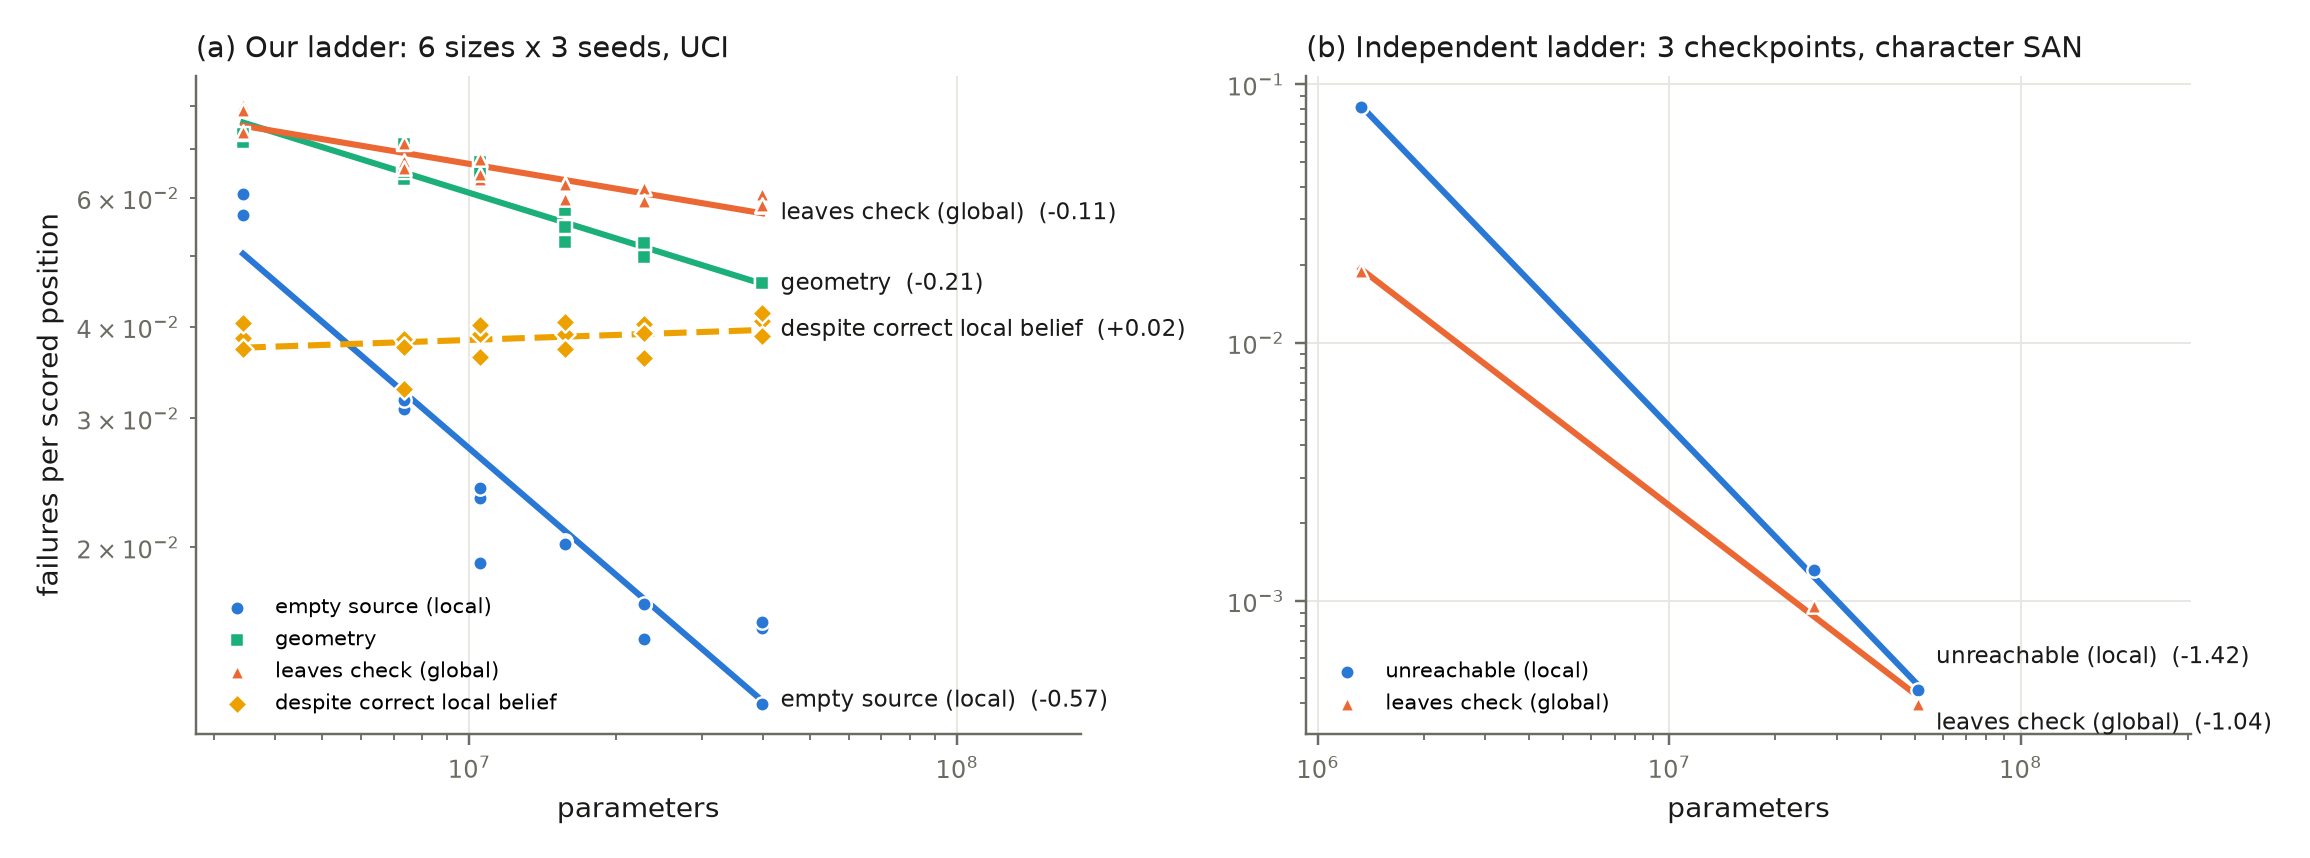
\includegraphics[width=\linewidth]{scaling.png}
\caption{Absolute failure rate against parameter count, log-log, so each line is a
power law and its slope, shown in each label, is the exponent. (a) Our ladder; each
point is one run. (b) An independent character-level ladder
(Section~\ref{sec:external}); each point is one checkpoint. In both, the local
class falls faster than the global one.}
\label{fig:scaling}
\end{figure}

Every class falls with size, so the result is not that larger models get worse at
anything. It is that they get better at different things at very different rates
(Table~\ref{tab:exponents}, Figure~\ref{fig:scaling}a). The exponents order
themselves by how local the rule is. Empty-source errors fall with exponent
$-$0.574; geometry, which depends on the squares between source and
destination, with $-$0.207; and check violations, which depend on
every attacker's position, with $-$0.112. The paired differential
between the check and empty-source exponents is +0.461
[+0.259, +0.599], positive in
100\% of rung resamples.

This is a claim about composition, and composition shifts accordingly. The
empty-source share of illegal moves falls from 0.230 to
0.110 while the check share rises from
0.307 to 0.448; geometry moves only from
0.285 to 0.335. The shift is
substantially one class collapsing into another rather than diffuse rebalancing.
Within models, check violations also concentrate at depth: their share rises from
early to late game in 6 of 6 rungs, from
0.260 to 0.519 at the largest.

Nothing in this section uses model internals. The measurement is a rules engine
and a move counter, which makes it reproducible against any chess model and immune
to objections about probe validity.

\paragraph{Why we do not extrapolate the fitted lines.}
The obvious next step is to extend the fitted lines beyond our largest model and
report what they imply at, say, one billion parameters. We did this in an earlier
version of this analysis and it is wrong, for a reason that applies to any
per-category scaling fit and that we have not seen stated.

The categories partition the illegal moves. Their absolute rates must therefore
sum to the illegal-move rate at every scale. Five independently fitted power laws
with five different exponents cannot satisfy that identity away from the fitted
range: the shallowest exponent must eventually dominate a total that is itself
falling faster. The failure is not gradual. Summing the independently fitted parts
and dividing by the independently fitted whole gives 1.02 at our
largest rung, which is fit noise, but 1.27 at one billion parameters
[1.13, 1.57, above one in
100\% of resamples] and 2.82 at one trillion.
Parts holding nearly three times the whole is not a wide estimate, it is an
arithmetic impossibility, and it means the extrapolation was never reporting the
exponents' implications at all. It is worth noting that the violation runs in the
direction that flatters our argument, since the categories we claim survive are
exactly the shallow ones that grow without bound.

\paragraph{A closed compositional fit.}
The repair is to fit the composition on the simplex rather than one category at a
time. The simplest repair is to stop fitting the aggregate and define it as the sum
of the categories, which satisfies the identity at every scale and keeps every
category exponent. Dividing through, the implied shares are a softmax linear in
$\log N$, so the compositional form and the derived total are the same model and
not a further choice. What the repair costs is the aggregate exponent: the derived
total is not a power law, and its effective slope drifts with scale. Coherence is not bought with fit quality. In range the closed model
attains RMSE 0.01251 across the 18 runs against
0.01322 for the uncoupled fits, so it is at least as good on the
data while being the only one of the two that can be extended.

Under the closed model the check category's share rises from 0.444
at our largest rung to 0.588 at one billion and 0.769
at one trillion, approaching but never exceeding 0.871, while the
locally decidable categories fall to 0.001. The paper's qualitative
claim is unchanged. What changes is that the projection is now bounded by
construction, so the figures above are statements the categories can jointly
satisfy, which the earlier ones were not.

The same discipline applies to the policy share, the fraction of illegal moves
occurring despite correctly decoded local belief. It is not a member of the
partition, since it cuts across the classes, but it is a proportion, and fitting a
proportion linearly in $\log N$ is unbounded in exactly the same way. Fitted on the
logit it rises from 0.308 at our largest rung to
0.596 at one billion and 0.951 at one trillion, having
been observed between 0.148 and 0.321. We report
it separately rather than folding it into the simplex; an earlier version of this
analysis did fold it in, which is wrong and which manufactured a spurious interior
maximum in the check category.

\paragraph{The failure is forced, not particular to us.}
Let the parts have exponents $a_i$ and the total exponent $b$, and let
$a^\star=\max_i a_i$. The sum of the parts is asymptotically $N^{a^\star}$ and the
total is $N^{b}$, so the ratio grows like $N^{a^\star-b}$ and diverges precisely
when $a^\star>b$. This is not a coincidence to be checked case by case. Fitted in
range, $b$ tracks the rate-weighted mean of the $a_i$, and a maximum is at least a
weighted mean, with equality only if every exponent is identical. Our own values
make the point: $a^\star$ is $-$0.112, the weighted mean is
$-$0.266, and the separately fitted $b$ is $-$0.267, giving
divergence +0.154. So any per-category scaling fit whose exponents
differ at all, which is the entire reason for reporting them separately, must
describe an impossibility beyond some finite scale. That scale is computable from
the reported exponents alone: ours passes a ten percent overspend at
174M parameters, well below the billion the earlier projection
used.

We checked this on a model family we did not train. Refitting Karvonen's ladder
over its own 4 classes gives divergence +0.234,
an overspend of 1.28 at one billion parameters, and a breakdown
scale of 243M. A different tokenisation, a different taxonomy,
a different training set and a different laboratory reproduce the defect at the
same order of magnitude, which is what the argument above predicts and what makes
us report it as a property of the method rather than of our data.

% ====================================================================
\section{External Validity}
\label{sec:external}

\paragraph{An independent ladder.}
Karvonen's lichess checkpoints \citep{karvonen2024emergent} differ from ours in
every respect we could change without training: character-level PGN rather than
one token per move, standard algebraic notation rather than UCI, roughly 16M
training games rather than ours, and different training code. We use its
1.3M, 25.8M, and 51.0M checkpoints
and read the model's move by greedy character decoding at move boundaries.

\paragraph{Verifying the adapters.}
Every step between an external model and our measurements fails silently rather
than with an error: a wrong vocabulary, a misaligned board, or a missed weight
transpose all yield plausible output. Each was therefore checked before use and
the checks rerun and recorded. The released weights ship without a tokenizer, so
the 32-character vocabulary was reconstructed and accepted only after
the model continued 3 of 3 standard openings
legally. Board state was aligned to the character before each move and verified
three ways at 4,081 sites, by independent replay, by re-parsing
the text prefix, and by the boundary character, with 0
disagreements. Checkpoints stored in a different weight layout were converted, and
all three trained checkpoints then played 20 of
20 moves legally from the opening, while the randomly initialised
control failed at its first move, as it should. A cached decoder used for speed
matched the uncached one at all 364 sites tested, the
algebraic-notation classifier passed 8 of 8
hand-written cases, and our OthelloGPT forward pass chose a legal move at
672 of 672 positions.

Algebraic notation changes the taxonomy in an instructive way. It never names a
source square, so the empty-source class cannot occur: a model that does not name
the square cannot place a piece on an empty one. The nearest local class is
\emph{unreachable}, no piece of the named type can reach the destination, which
also absorbs path blocking. That makes the local class less local than ours and
biases the comparison against the result.

The ordering holds (Table~\ref{tab:external}, Figure~\ref{fig:scaling}b).
Unreachable errors fall with exponent $-$1.415 and check violations with
$-$1.044, a differential of +0.371, against +0.461 on
our ladder. The local share of failures falls from 0.654 to
0.377 while the check share rises from 0.152 to
0.334. Within the smallest checkpoint the check share rises from
0.060 to 0.266 across depth while the unreachable
share falls from 0.730 to 0.553. At comparable size
this ladder fails far less often than ours, because it was trained on far more
data, so only exponents are comparable and never levels.

\begin{table}[t]
\centering\small
\caption{Independent ladder. Absolute rates per scored position. With three
checkpoints no uncertainty in the fit itself can be estimated; the intervals
propagate only each checkpoint's sampling noise in class shares and should be read
as a lower bound on uncertainty, not as a confidence statement about the slope.}
\label{tab:external}
\begin{tabular}{lcccc}
\toprule
checkpoint & illegal & failures & unreachable & leaves check \\
\midrule
1.3M     & 0.1253     & 2,836     & 0.08193     & 0.01901 \\
25.8M   & 0.0028   & 233   & 0.00132   & 0.00095 \\
51.0M & 0.0012 & 101 & 0.00045 & 0.00040 \\
\midrule
exponent & & & $-$1.415 [$-$1.482, $-$1.365] & $-$1.044 [$-$1.121, $-$0.978] \\
\bottomrule
\end{tabular}
\end{table}

\paragraph{A game with non-local rules.}
Othello legality is non-local by construction: a move is legal only if it flanks a
line of opponent discs, so it is never decidable from the target square. There is
no published Othello ladder, so no exponent can be fitted, and we test only what
the claim implies for a single well-trained model: that its residual failures
should be the non-local kind. In Li's synthetic OthelloGPT \citep{li2023emergent},
across 211,815 positions and 161 failures, 0
are moves onto an occupied square and 160 are moves that flank
nothing. The comparison is weaker than it looks, because discs never leave a
square: whether a square is occupied reduces to whether it appears in the move
history, which requires no state tracking at all. Failures also concentrate late,
6, 32, and 123 across the three move
bands.

\paragraph{Heavy training.}
The mechanism in Section~\ref{sec:mech} rests on three measurements taken on
models trained on about a hundred thousand games. We repeated all three on
Karvonen's character-level model trained on roughly 16M games
(Table~\ref{tab:chessgpt}). Its board state at depth is better than ours, so the
comparison is not against a model whose state was hard to extract: probe accuracy
on occupied squares is 0.731 early and 0.315 late,
against 0.777 and 0.167 for ours. Human games give
only 131 illegal moves, so we also report uniformly random legal play,
which lifts the illegal rate from 0.0026 to 0.0231.

\begin{table}[t]
\centering\small
\caption{The three mechanism measurements on a model trained on roughly 16M games.
Belief consistency is the fraction of illegal moves legal on the probe-decoded
board. The AUC on our models is a mean over depth buckets and on Chess-GPT is
pooled over depth, which is not the same quantity; only the sign and rough size of
the move-touched advantage are compared. Chess-GPT's move-touched square is the
destination, since algebraic notation names no source.}
\label{tab:chessgpt}
\begin{tabular}{lccc}
\toprule
& ours & Chess-GPT, human & Chess-GPT, random play \\
\midrule
belief consistency, own board & 0.355 & 0.122 & 0.188 \\
\quad mismatched board        & 0.050 & 0.038 & 0.061 \\
\quad random move             & 0.007 & 0.000 & 0.003 \\
\quad own / mismatched        & 7.2 & 3.2 & 3.1 \\
\midrule
AUC, whole board              & 0.587 & 0.530 & 0.485 \\
AUC, move-touched             & 0.647 & 0.608 & 0.552 \\
\quad advantage               & +0.060 & +0.078 & +0.068 \\
\midrule
edit, state direction         & n/a & $-$0.078 & $-$0.042 \\
edit, norm-matched random     & & $-$0.005 & $-$0.005 \\
edit, manipulation check      & & 1.000 & 1.000 \\
\bottomrule
\end{tabular}
\end{table}

All three hold, at reduced size. The model's illegal moves are legal on its own
decoded board far more often than on another position's, at a ratio of
3.1 against 7.2 for ours. Fidelity at the square
the move targets predicts illegality where whole-board fidelity is near chance.
And emptying a square in the model's belief lowers the probability of moves from
it, by $-$0.037 [$-$0.050, $-$0.026] beyond a
norm-matched random edit, with the decoded square flipped in 1.000 of
cases. Heavy training weakens coherent error without removing it.

% ====================================================================
\section{Mechanism}
\label{sec:mech}

Why does scale leave the global class behind? Three measurements, using the probe
and edit instruments of \priort, point to the same answer.

\paragraph{Coupling is local.}
We repair the model's belief at the squares its illegal move touches by adding
probe-derived occupancy directions to the residual stream, and score the change in
a forced-choice preference $r = P(m^\ast)/(P(m^\ast)+P(m_{\mathrm{ill}}))$ between
the best legal move and the illegal one, which is invariant to uniform flattening
of the distribution. Two controls matter. A wrong-target edit installs the same
occupancy at an unrelated square; an irrelevant edit spends an identical budget on
squares that are wrongly decoded but not touched by the move. Both are matched to
correct repair in magnitude and construction, and all contrasts are taken on
positions where the two edits changed the output entropy comparably. Across
18 models, correct repair beats wrong-target in
18 (sign test $7.6\times10^{-6}$) and beats the irrelevant edit in
18 ($7.6\times10^{-6}$), mean advantage +0.039. Only
11 of the irrelevant-edit contrasts exclude zero individually,
because matching retains about half the positions per run; the evidence is that
none of 18 is negative. Correcting the squares the move depends on
changes behaviour more than correcting other wrong squares, which reconciles a
weak whole-board coupling \citep{balogh2026verification} with a strong local one.

\paragraph{Correction reaches about two squares.}
The repair channel works: when we corrupt a single square ourselves and repair it,
the model recovers a legal move in 0.733 [0.699,
0.770] of cases against 0.253 for a random repair. On the
model's own failures, repair at the touched squares restores a legal move in only
0.114, a 6.4-fold gap. Natural failures involve a
median of 14 wrongly decoded squares, so we tried repairing all
of them. It fails in a specific way (Table~\ref{tab:mechanism}): a two-square edit
restores the decoded value at 0.677 of its targets, while an
all-square edit restores 0.304, and full strength per square does
no better at 0.279. Whole-board repair lowers occupied-square
decoding accuracy from 0.326 to 0.185. The instrument
has a capability limit of roughly two squares, whatever the edit magnitude.

\begin{table}[t]
\centering\small
\caption{Mechanism summary. Meta rows count models out of 18;
repair and fidelity rows are from a single model.}
\label{tab:mechanism}
\begin{tabular}{lc}
\toprule
correct beats wrong-target edit, models          & 18 / 18 \\
correct beats irrelevant-square edit, models     & 18 / 18 \\
\midrule
induced single-square corruption, recovered      & 0.733 \\
\quad random repair                               & 0.253 \\
natural failures, recovered by touched-square repair & 0.114 \\
\midrule
decoded value restored, two-square edit          & 0.677 \\
decoded value restored, all-square edit          & 0.304 \\
occupied-square accuracy, before and after all-square edit & 0.326 to 0.185 \\
\bottomrule
\end{tabular}
\end{table}

\paragraph{What local correction cannot reach.}
Where decoded belief is already correct at both squares a move touches, a check
violation accounts for 0.477 of failures on average against
0.286 for geometry, and is the largest class in
15 of 18 models. Such failures cannot be attributed
to the decoded belief being wrong at the move's squares, and a check violation is
decided by squares an edit of two cannot address. Their
absolute rate is flat with size, exponent +0.023
[$-$0.005, +0.066], a differential against
empty-source errors of +0.596 [+0.367, +0.761].
An earlier oracle-free attempt to repair state by re-presenting information the
model already attends to also failed, leaving the late-game illegal rate at
0.295 against 0.296 without intervention.

We do not claim these failures are unrepairable in principle. The instrument cannot
install a multi-square correction, so whether the residual is genuine policy
failure or simply beyond its reach is undetermined, and we recorded the stronger
reading as retracted (Appendix~\ref{app:integrity}). The claim is narrower and
sufficient: the component scale leaves behind is concentrated in exactly the
failures that correction at the move's squares cannot address.

% ====================================================================
\section{The Standard Metric Inverts}
\label{sec:inversion}

Interventions on state are usually scored by whether the model's output becomes
legal. On our repair edits that metric orders the conditions nearly in reverse
(Table~\ref{tab:inversion}). On one model, correct repair produces the largest
preference shift, +0.140, and a random direction the smallest,
+0.041; yet after the edit the random direction leaves a legal top-1 move
in 0.268 of cases and correct repair in 0.147. The random
direction also raises output entropy most, by +0.298. Hedging moves
probability off a confidently illegal move and onto whatever else is plausible,
some of which is legal.

\begin{table}[t]
\centering\small
\caption{Repair conditions on one model (600 positions, 61
games): change in forced-choice preference, fraction of top-1 moves legal after
the edit, change in entropy, and how often the target square's decoded value
flipped. The null edit re-installs values already decoded correctly and is zero by
construction.}
\label{tab:inversion}
\begin{tabular}{lcccc}
\toprule
condition & $\Delta r$ & legal after edit & $\Delta$ entropy & decode flipped \\
\midrule
correct repair   & +0.140 & 0.147 & $-$0.017 & 0.826 \\
irrelevant squares & +0.061   & 0.203     & $-$0.177     & 0.163 \\
wrong target     & +0.053   & 0.037   & $-$0.007   & 0.171 \\
random direction & +0.041    & 0.268    & +0.298    & 0.080 \\
null             & 0.000    & 0.000    & 0.000    & 0.000 \\
\bottomrule
\end{tabular}
\end{table}

This is not one model. In 18 of 18 models the random
direction produces more legal moves than correct repair while correct repair
produces the larger preference shift (sign test $7.6\times10^{-6}$), and the random
direction has the best legal-move rate of all four edits in 16 of
them.
Its advantage in legal moves over correct repair ranges from +0.048 to
+0.143.

The same artefact affects our own preference metric if uncontrolled. The raw
advantage of correct repair over wrong-target is +0.087; restricted to
positions where both edits changed entropy comparably it is +0.036
[+0.011, +0.058], 2.4 times smaller. The
edit also responds gradedly to strength: preference rises from +0.042 at a
quarter of calibrated strength to +0.140 at calibrated strength, then
turns to $-$0.046 and $-$0.091 at double and quadruple, a
rise-then-collapse that is harder to explain as generic damage than a monotone
decline would be.
Studies that score state interventions by illegal-move rate, or by any error rate
a flatter distribution can lower, may be measuring hedging.

% ====================================================================
\section{Discussion}

The practical content is about where effort goes. The class that does not fall
with size is the one defined by constraints spanning the whole board, and on our
evidence it is also the class that correcting the model's belief about a move's own
squares does not reach. We read this, as an interpretation we have not tested
directly, as a caution for interventions such as auxiliary board losses and state
supervision: they aim at the model's knowledge of where pieces stand, and the
failures most directly attributable to that knowledge are the ones scale is already
removing. An intervention that lowers total error while leaving the global class
flat may have improved only what scale improves anyway, and should be evaluated by
its effect on that class.

This also bounds what an intervention study can show. A training comparison that
targets state-attributable failure is adequately powered on our data, detecting a
change of 19\% of that component with seed variation contributing
little (relative spread 0.028), but the component is a small share of
what goes wrong, so a detectable improvement is a small behavioural one.

A methodological point generalises further than our subject. Whenever failures are
decomposed into categories and each category is given its own scaling exponent, the
fits sit alongside a separately fitted aggregate, the two make claims that cannot
both hold, and extrapolation is where the conflict becomes visible. The check costs nothing: sum the extrapolated parts and see whether they
still make the whole. We report it because our own uncoupled fits passed every gate
in this paper, agreed with the data in range, and were still projecting an
impossibility two orders of magnitude out. Any decomposition of error into
categories that scale at different rates, whether by capability, benchmark subset,
or error type, has this property, and fitting on the simplex removes it without
costing accuracy. We supply the check as \texttt{code/closure\_check.py}, which
needs only the exponents and intercepts such papers already print.

One consequence is easy to miss, and we missed it. An inadmissible fit voids
negative conclusions as well as positive ones. While preparing this section we
tested whether failure composition is governed by achieved competence rather than
by size, rejected it because the fitted shares exceeded one, and recorded it as
refuted. That rejection was worthless: predicting an impossibility is what the
uncoupled form does everywhere, so its disagreement with data carries no evidence
about the hypothesis under test. Refitting the same comparison on the simplex, in
competence coordinates, and predicting Karvonen's checkpoints out of sample does
refute it, by a total variation distance of 0.490 against
0.100 for size coordinates and 0.115 for predicting our
own mean composition. The conclusion survived; the first argument for it did not.
A model that cannot make an admissible prediction cannot be used to reject
anything.

The local and global distinction is not specific to chess. Wherever a checker can
say not only that a step is wrong but which constraint it violated, program
execution, spreadsheet recalculation, and formal proof among them, the same
decomposition is available, and the question of which violations scale removes can
be asked without any access to model internals.

% ====================================================================
\section{Limitations}
\label{sec:limits}

\begin{description}[nosep]
\item[Depth and width are confounded.] Both ladders grow depth and width together,
so an exponent in parameters does not isolate either.
\item[Three external checkpoints.] The independent ladder supports directional
agreement, not a second estimate of the slope; its intervals omit fit uncertainty.
\item[Notation changes the classes.] Algebraic notation removes the empty-source
class, and its nearest local analogue absorbs path blocking.
\item[Othello cannot test scaling.] No ladder exists, and its local class requires
no state tracking, so it is a consistency check rather than a replication.
\item[Consistency is not validation.] The derived total guarantees the
projection is arithmetically possible, which the uncoupled fits are not. It does
not make it observed: every scale past 39.9M is extrapolation, and
a different link satisfying the same constraint would give different numbers while
agreeing that the uncoupled ones are inadmissible.
\item[The check class is not an exact power law.] Fitting it quadratically in
$\log N$ gives a curvature term whose bootstrap interval excludes zero, so the
exponent we report for it is a local slope over our range. This does not change its
sign, its separation from the local classes, or the ordering that is this paper's
result, all of which are about the fitted range. It does mean a reader should not
extend that one exponent far beyond the ladder.
\item[The residual is unattributed.] The repair instrument corrects about two
squares, so whether failures despite correct local belief reflect policy or
unreachable state is undetermined.
\item[Probe-based rows depend on a linear probe.] A nonlinear decoder of four times
the capacity gains only +0.011 to +0.033 across depth
(Appendix~\ref{app:capacity}), so decoder weakness does not explain decay, but the
probe-based rows inherit its approximation. The headline result uses no probe.
\item[One game family.] Chess and Othello both carry exact oracles, which is what
makes them measurable and what makes them unrepresentative of open-ended reasoning.
\end{description}

% ====================================================================
\section{Conclusion}

Scale does not remove long-horizon errors evenly. In chess transformers it removes
errors decidable from a move's own squares several times faster than errors
decided by the whole board, the ordering replicates on an independent model family,
and the failures that occur despite correctly decoded belief at the move's squares
do not decline at all. The measurement needs only a rules engine. What it suggests is that the
failures worth studying at scale are the ones defined by global constraints, and
that interventions should be judged by their effect on those, measured with a
metric a flatter output distribution cannot improve.

\section*{Declarations}

\paragraph{Disclosure statement.}
 The authors report no conflict of interest. 

\paragraph{Funding.}
 This research received no specific grant from any funding agency in the
public, commercial, or not-for-profit sectors. 

\paragraph{Data availability statement.}

The analysis code, every result file cited by the manuscript, and the macro
provenance record are available at
\url{https://github.com/MohitPratapSinghRathore/derived-total}. Trained checkpoints
are available from the corresponding author on reasonable request, being too large
to distribute with the repository. External checkpoints are public.


\paragraph{AI usage declaration.}
During preparation the authors used a generative AI tool to assist with analysis
code and language editing. The authors reviewed and edited all output and take full
responsibility for the content.

\appendix

\section{Probe capacity}
\label{app:capacity}

Every fidelity curve in this line of work is read with a linear probe, which could
confound information leaving the representation with information becoming
nonlinearly encoded. On identical activations and budgets, a two-layer probe whose
hidden layer is four times the residual width improves occupied-square accuracy by
between
+0.011 and +0.033 across depth, with no tendency to widen.
The same nonlinear probe reaches 0.000 on a control task with
shuffled boards and 0.015 on a randomly initialised model in the
deepest bucket, so there is no memorisation headroom for extra capacity to exploit.
Decay in these curves is therefore not explained by the weakness of a linear
decoder, though a single alternative decoder cannot rule out every nonlinear
encoding.

\section{Integrity record}
\label{app:integrity}

The analysis was pre-registered (SHA-256 prefix \texttt{28b68e5200dc0dba}).
Three amendments changed reported claims and are stated here in full. First, the
frozen entropy-matching procedure was vacuous, since weighting strata by their own
counts reproduces the overall mean; it was replaced by matching on positions after
point estimates were seen, and the replacement reduced the headline effect. Second,
a prior that about a third of illegal moves would be restored to legality by repair
was mis-specified, by conflating whether an error is explicable by wrong belief with
whether repairing belief is sufficient to change behaviour; the observed rate was
far lower. Third, a conclusion that the failures repair could not fix are genuine
was retracted once whole-board repair was shown not to install a board, which is
why Section~\ref{sec:mech} leaves that residual unattributed.

Two further corrections changed how a result was stated rather than a reported
value. The scaling result was first framed in terms of shares of failures, and that
framing was stated before it was found to imply that models grew worse at a class
they were in fact improving at; it was revised to absolute rates, which is the form
reported here. The metric comparison was first reported on one model and is now
reported across all of them. Analysis corrections that changed no reported claim,
including a move-touched definition that scored illegal algebraic moves at
arbitrary squares and edit intervals clustered on too few games, are recorded in the
analysis repository's version history.

\nocite{rathore2026coherent}
\bibliographystyle{apalike}
\bibliography{refs}

\end{document}
